\section{Resoconto delle attività di verifica}
In questa appendice vengono esposti gli esiti delle attività di verifica svolte sui documenti e sul codice consegnati nelle varie revisioni.
\subsection{Revisione dei requisiti}
\subsubsection{Analisi statica dei documenti}
L'analisi statica dei documenti è stata eseguita mediante Walkthrough\textsubscript{\textbf{G}}. In questo modo sarà possibile applicare Inspection\textsubscript{\textbf{G}} successivamente.
\subsection{Revisione di progettazione}
\subsubsection{Analisi statica dei documenti}
L'analisi statica della documentazione ha seguito il procedimento descritto nella sezione §B.1.1., la quale ha garantito un'attività di Inspection\textsubscript{\textbf{G}} più mirata.\\
Come supporto alla stesura della documentazione il gruppo ha deciso di utilizzare il plugin \textit{Code Spell Check} per l'editor \textit{Visual Studio Code}. Questo ha permesso un maggior controllo e
una riduzione significativa degli errori.
\subsubsection{Analisi statica del codice}
La stesura del codice è supportata da \textit{ESLint v7.24.0}, linter per il linguaggio TypeScript. Questo ha aiutato nella stesura di codice di codice uniforme e sintatticamente corretto.
\subsection{Metriche}
Alcune metriche verranno calcolate successivamente con l'avanzare del progetto.\\
I dati riportati nel seguito fanno riferimento a:
\begin{itemize}
    \item \textbf{A:} fase di analisi;
    \item \textbf{C:} fase di consolidamento dei requisiti;
    \item \textbf{PA:} fase di progettazione architetturale;
    \item \textbf{PD:} fase di progettazione di dettaglio (da aggiungere con l'avanzare del progetto);
    \item \textbf{VC:} fase di validazione e collaudo (da aggiungere con l'avanzare del progetto).
\end{itemize}
\newpage
\subsubsection{MPR04 - EAC (Estimate at Completion)}
\begin{figure}[!ht]
    \caption{Estimate at Completion}
    \vspace{10px}
    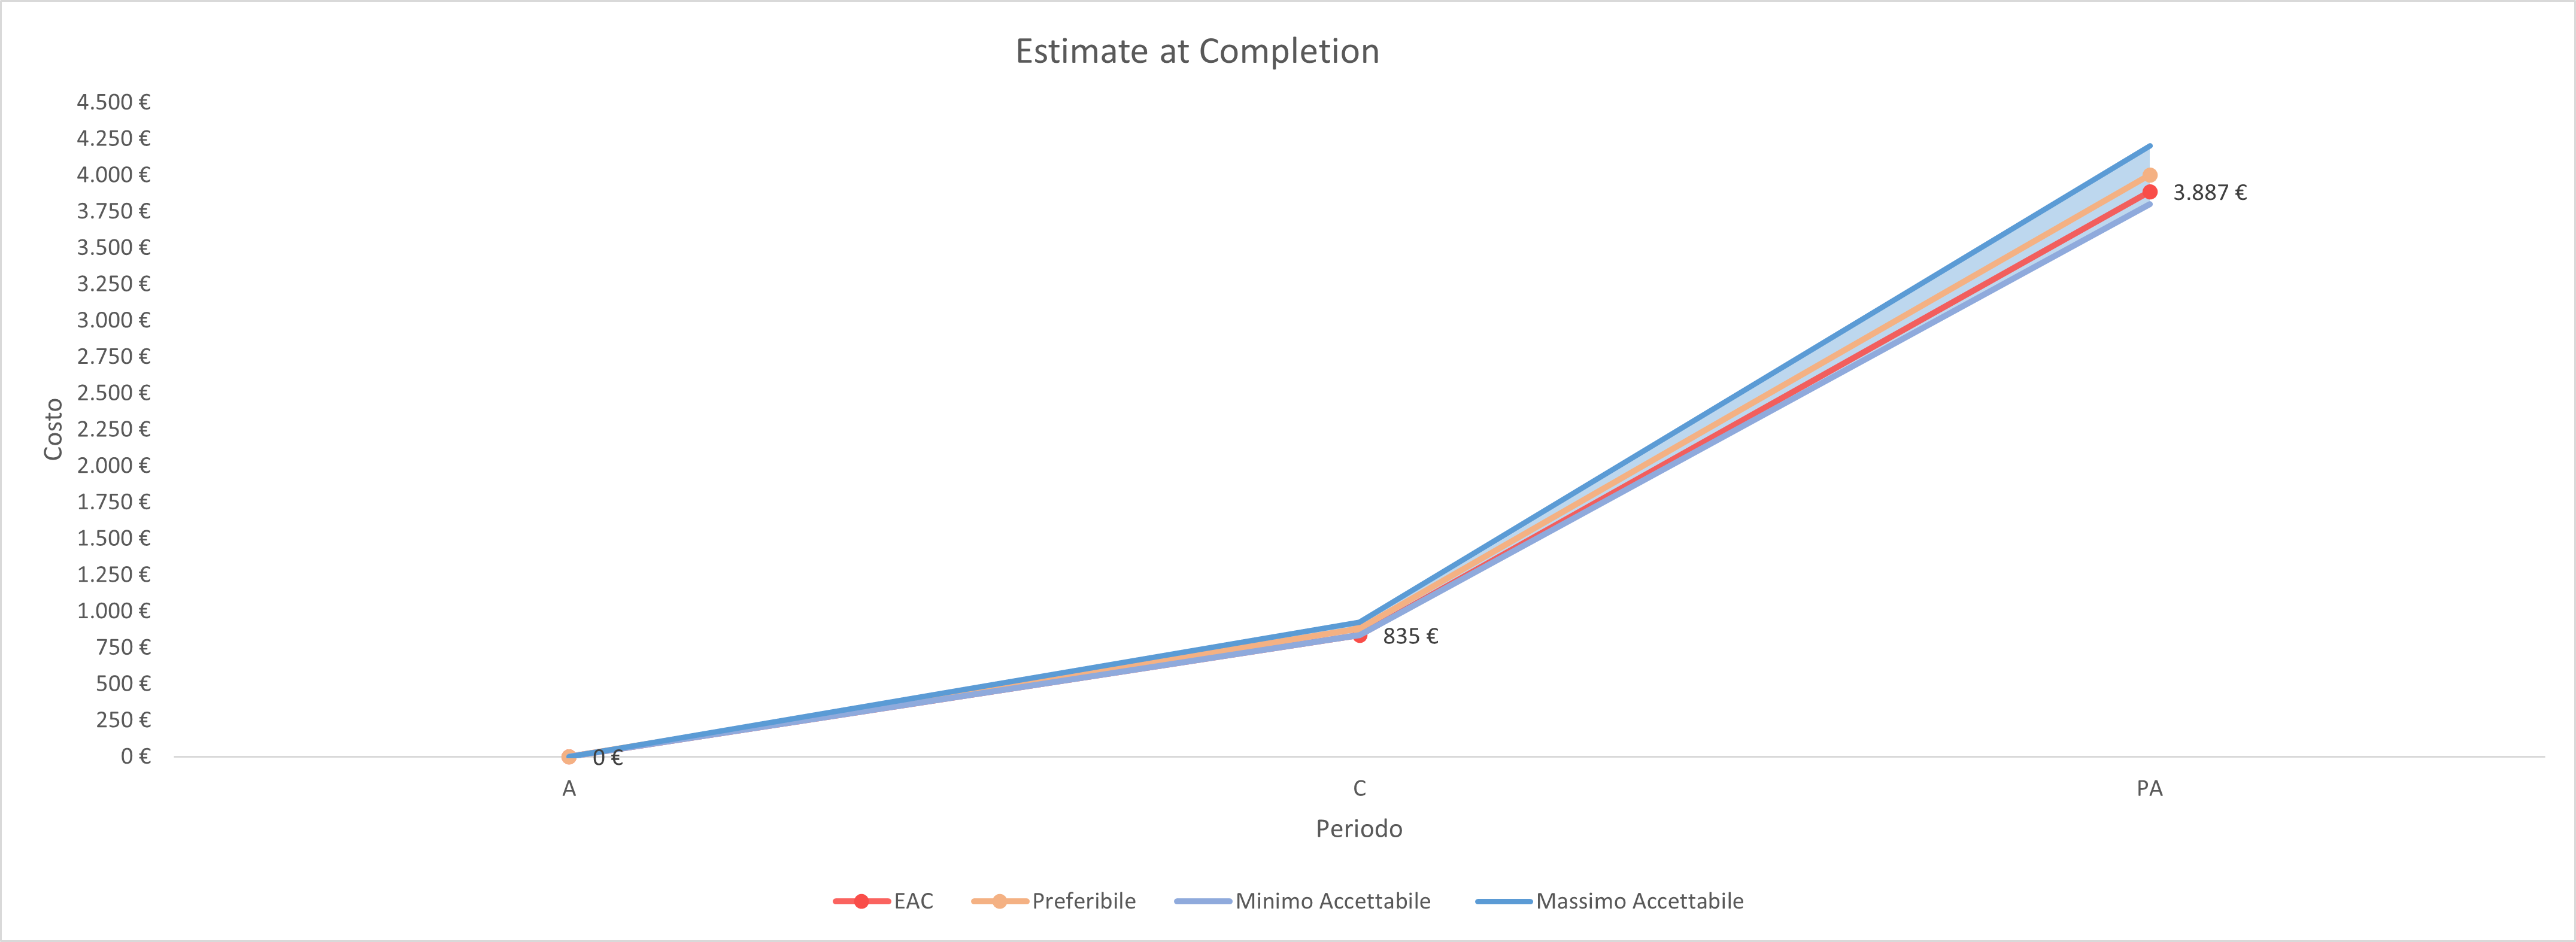
\includegraphics[scale=0.5]{sezioni/immagini/EstimateAtCompletion.png}
    \centering
\end{figure}
\subsubsection{MPR05 - VAC (Variance at Completion)}
\begin{figure}[!ht]
    \caption{Variance at Completion}
    \vspace{10px}
    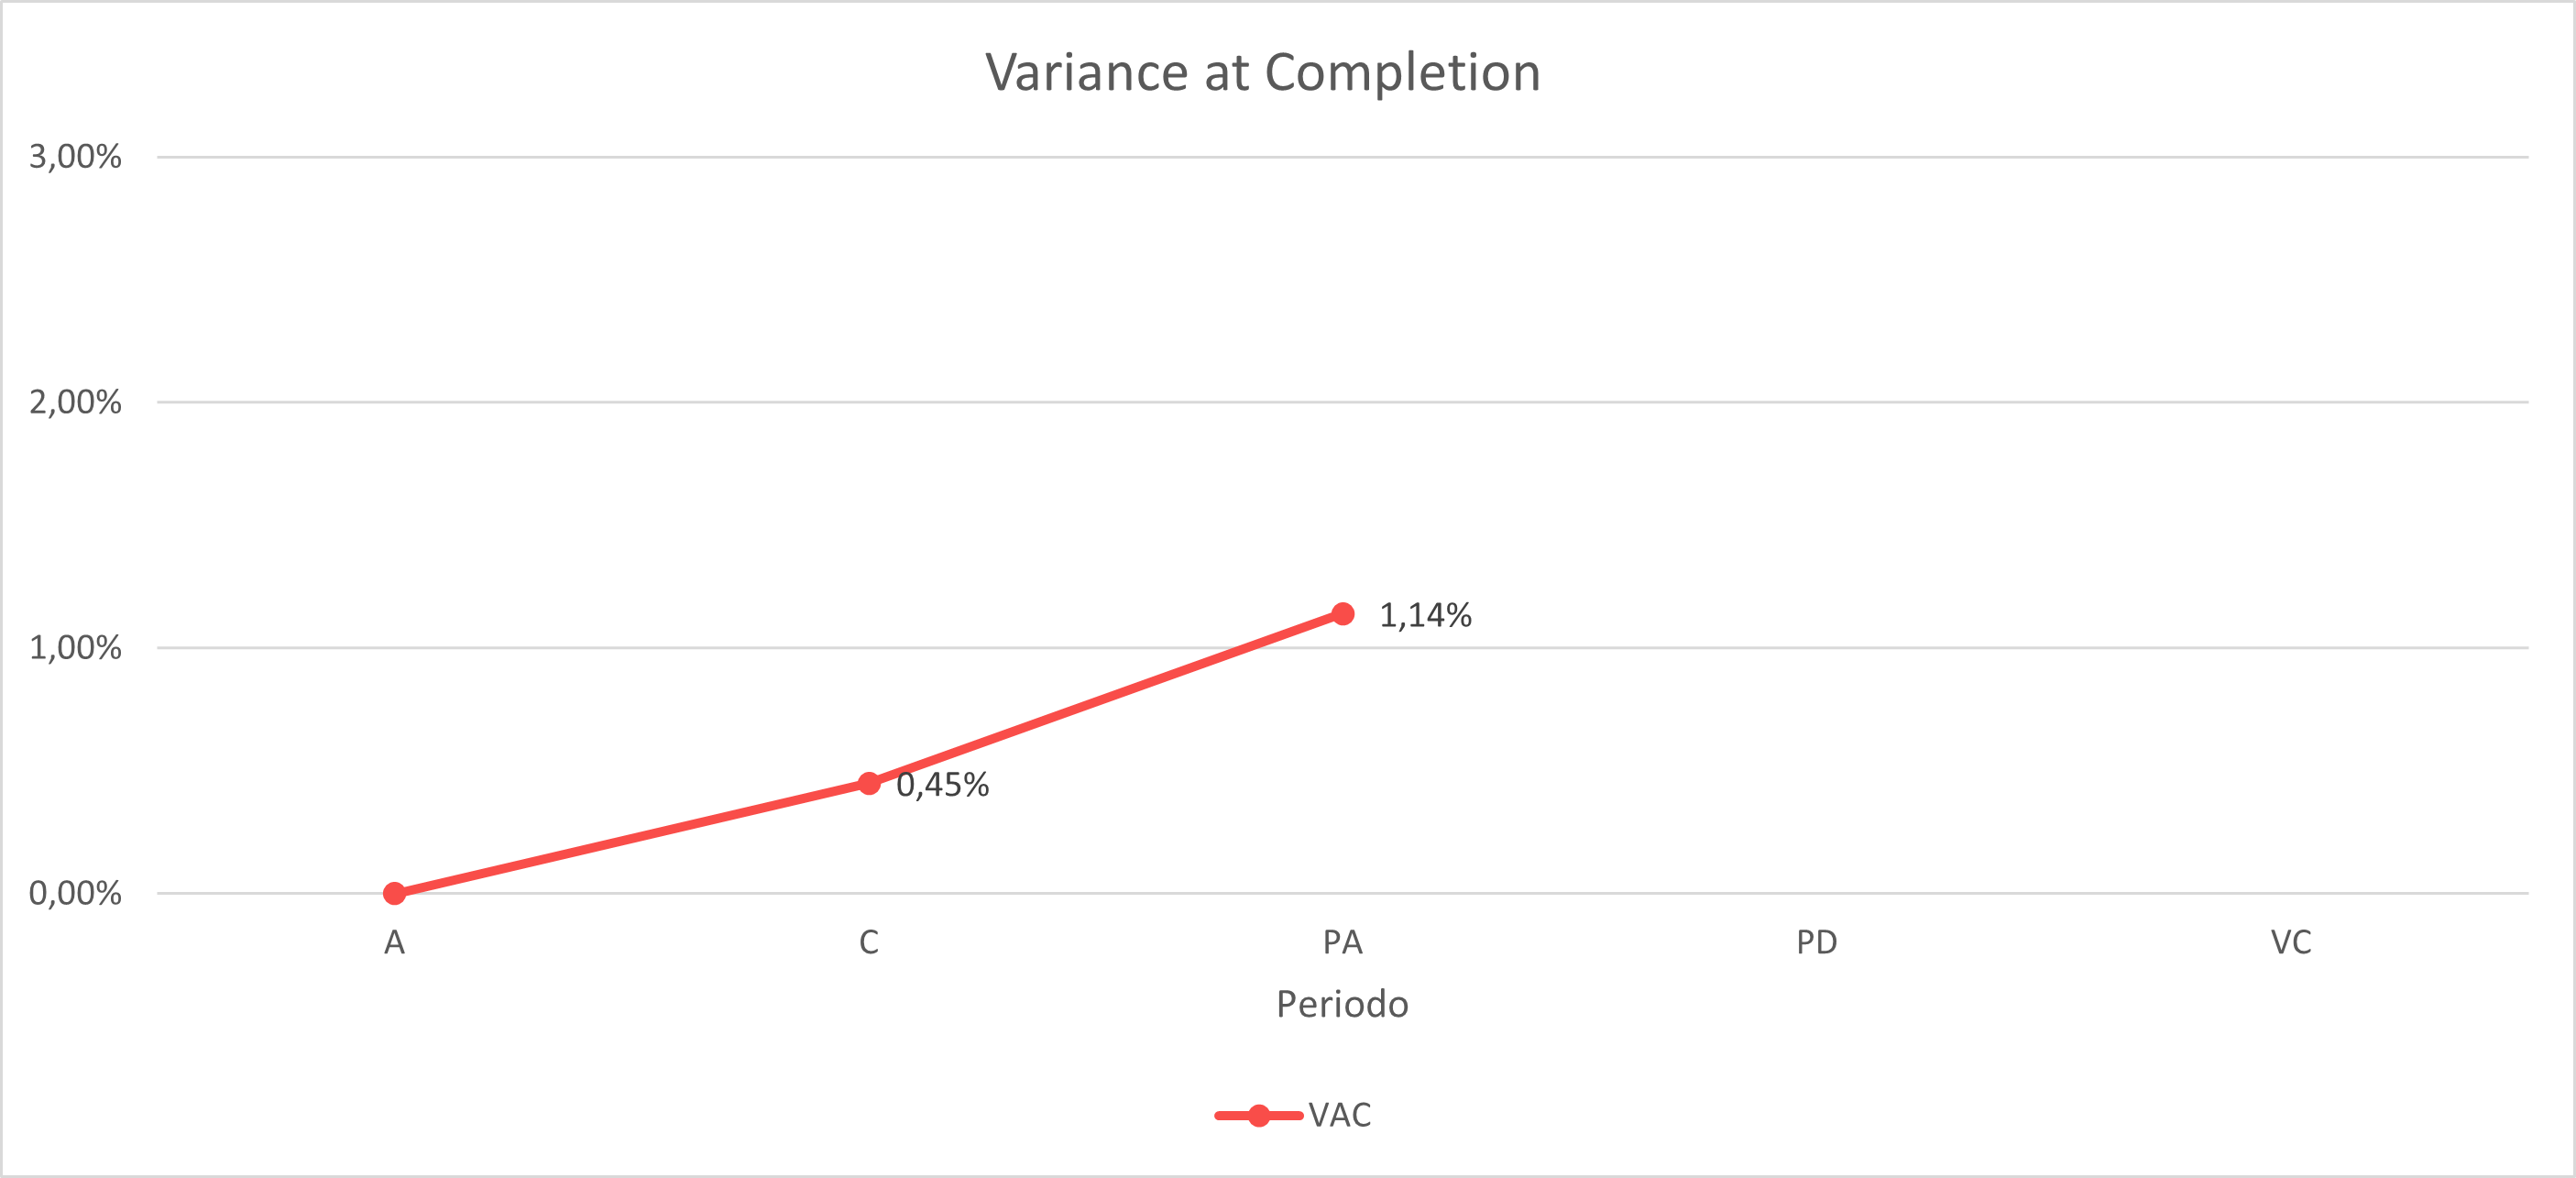
\includegraphics[scale=0.5]{sezioni/immagini/VarianceAtCompletion.png}
    \centering
\end{figure}
\pagebreak
\subsubsection{MPR06 - AC (Actual Cost)}
\begin{figure}[!ht]
    \caption{Actual Cost}
    \vspace{10px}
    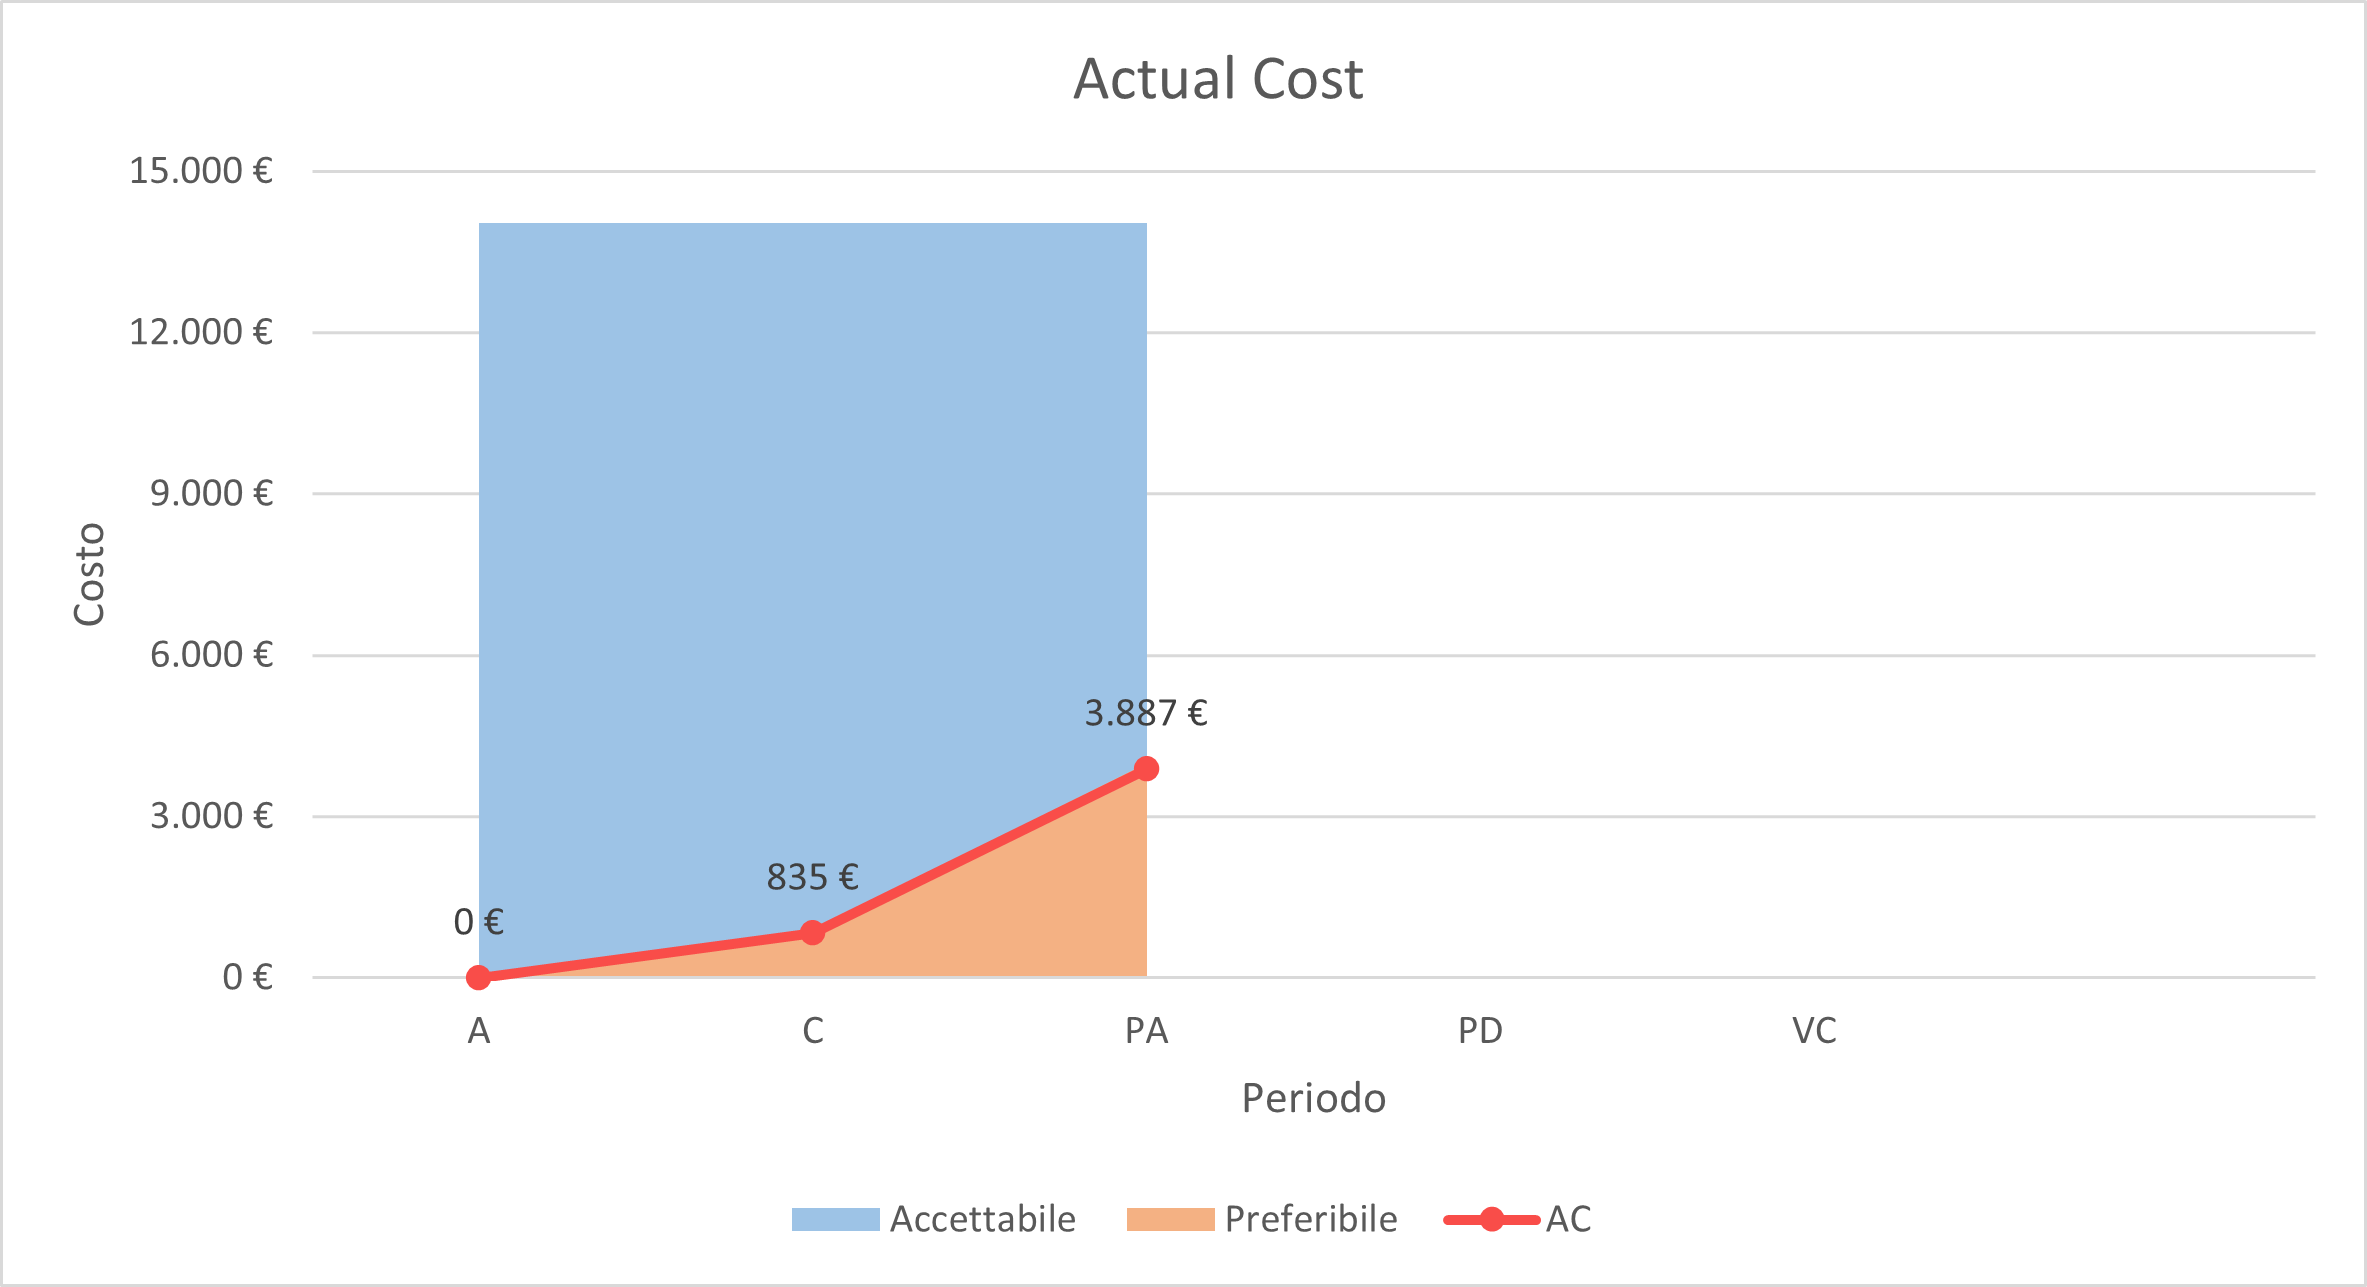
\includegraphics[scale=0.5]{sezioni/immagini/ActualCost.png}
    \centering
\end{figure}
\subsubsection{MPR08 - BV (Budget Variance)}
\begin{figure}[!ht]
    \caption{Budget Variance}
    \vspace{10px}
    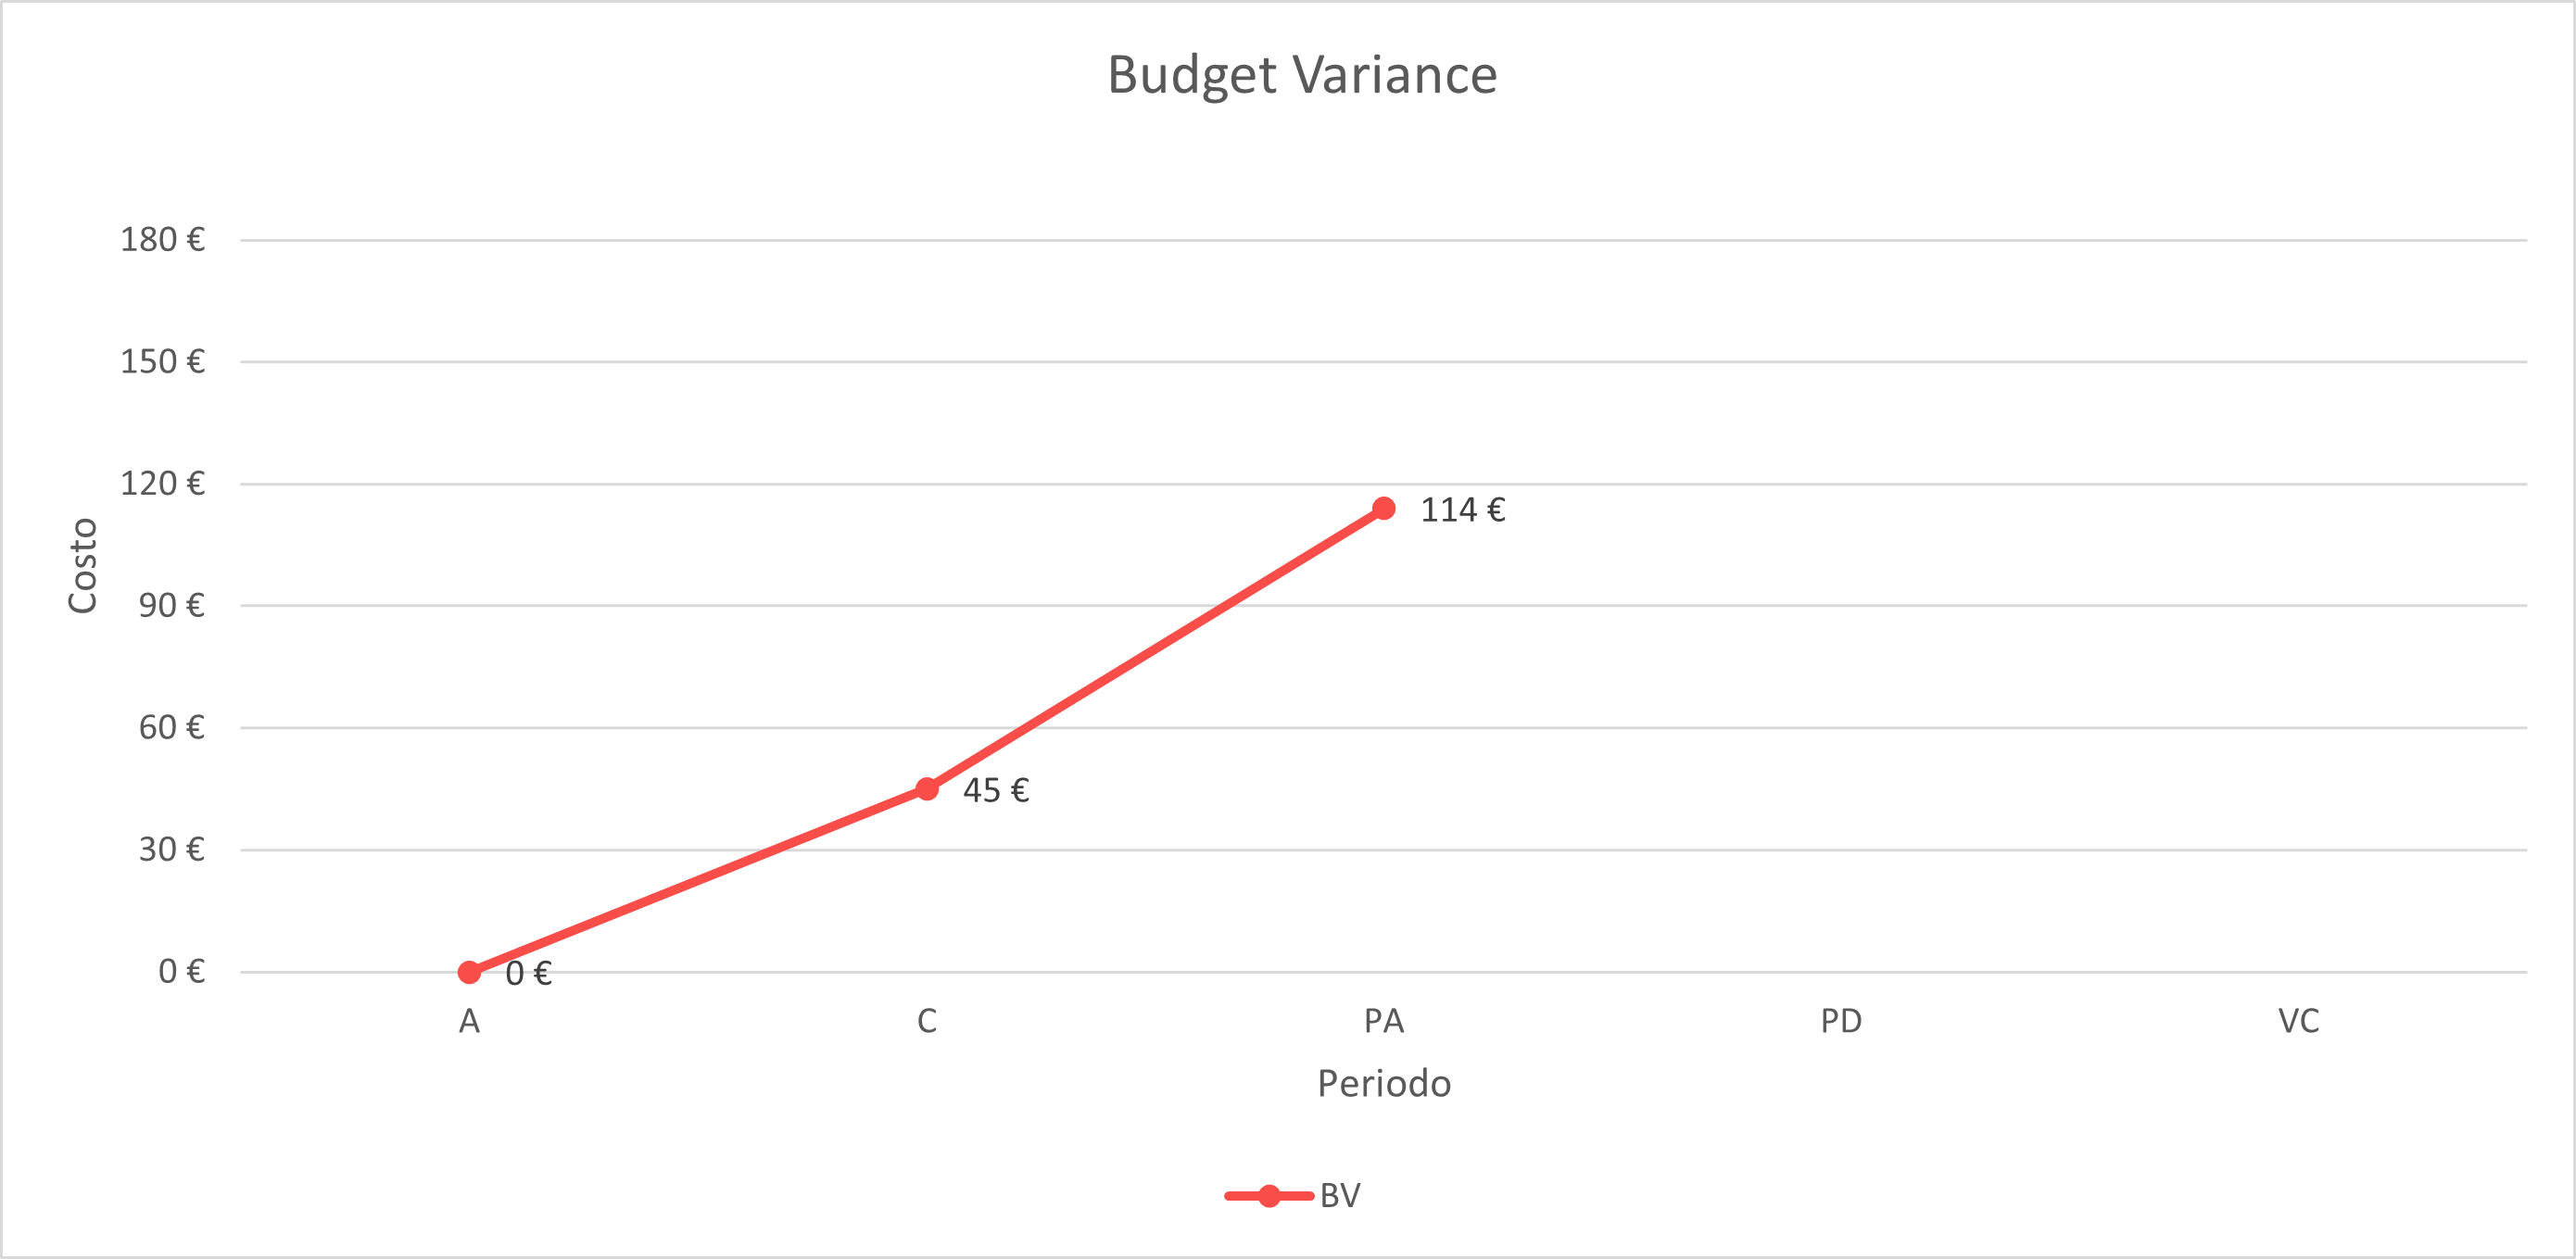
\includegraphics[scale=0.5]{sezioni/immagini/BudgetVariance.png}
    \centering
\end{figure}
\pagebreak
\subsubsection{MPR10 - Indice di Gulpease}
\subsubsubsection{Andamento complessivo}
\begin{center}
    \centering
    \rowcolors{2}{logo!10}{logo!40}
    \renewcommand{\arraystretch}{1.8}
    \label{tab:IndiciGulpease}
    \begin{longtable}[!h]{p{100px} p{50px} p{50px} p{50px} p{50px} p{50px} p{50px}}
        \caption{Esiti verifica con Gulpease}                                                                                        \\
        \rowcolor{logo!70}   \textbf{Documento} & \textbf{A} & \textbf{C} & \textbf{PA} & \textbf{PD} & \textbf{VC} & \textbf{Esito} \\
        \textit{Norme di Progetto}              & 68         & 68         & 72          & /           & /           & Superato       \\
        \textit{Piano di Progetto}              & 73         & 73         & 69           & /           & /           & Superato       \\
        \textit{Analisi dei Requisiti}          & 71         & 71         & 66          & /           & /           & Superato       \\
        \textit{Piano di Qualifica}             & 69         & 69         & 67           & /           & /           & Superato       \\
        \textit{Studio di Fattibilità}          & 74         & 74         & /           & /           & /           & Superato       \\
        \textit{Glossario}                      & 49         & 49         & 49           & /           & /           & Superato       \\
        \textit{Verbali interni (media)}        & 67         & 67         & 56           & /           & /           & Superato       \\
        \textit{Verbali esterni (media)}        & 71         & 71         & 51           & /           & /           & Superato       \\
        \rowcolor{white}
    \end{longtable}
\end{center}
\subsubsubsection{Andamento per documento}
\begin{figure}[!ht]
    \caption{Indice di Gulpease: \textit{Norme di Progetto}}
    \vspace{10px}
    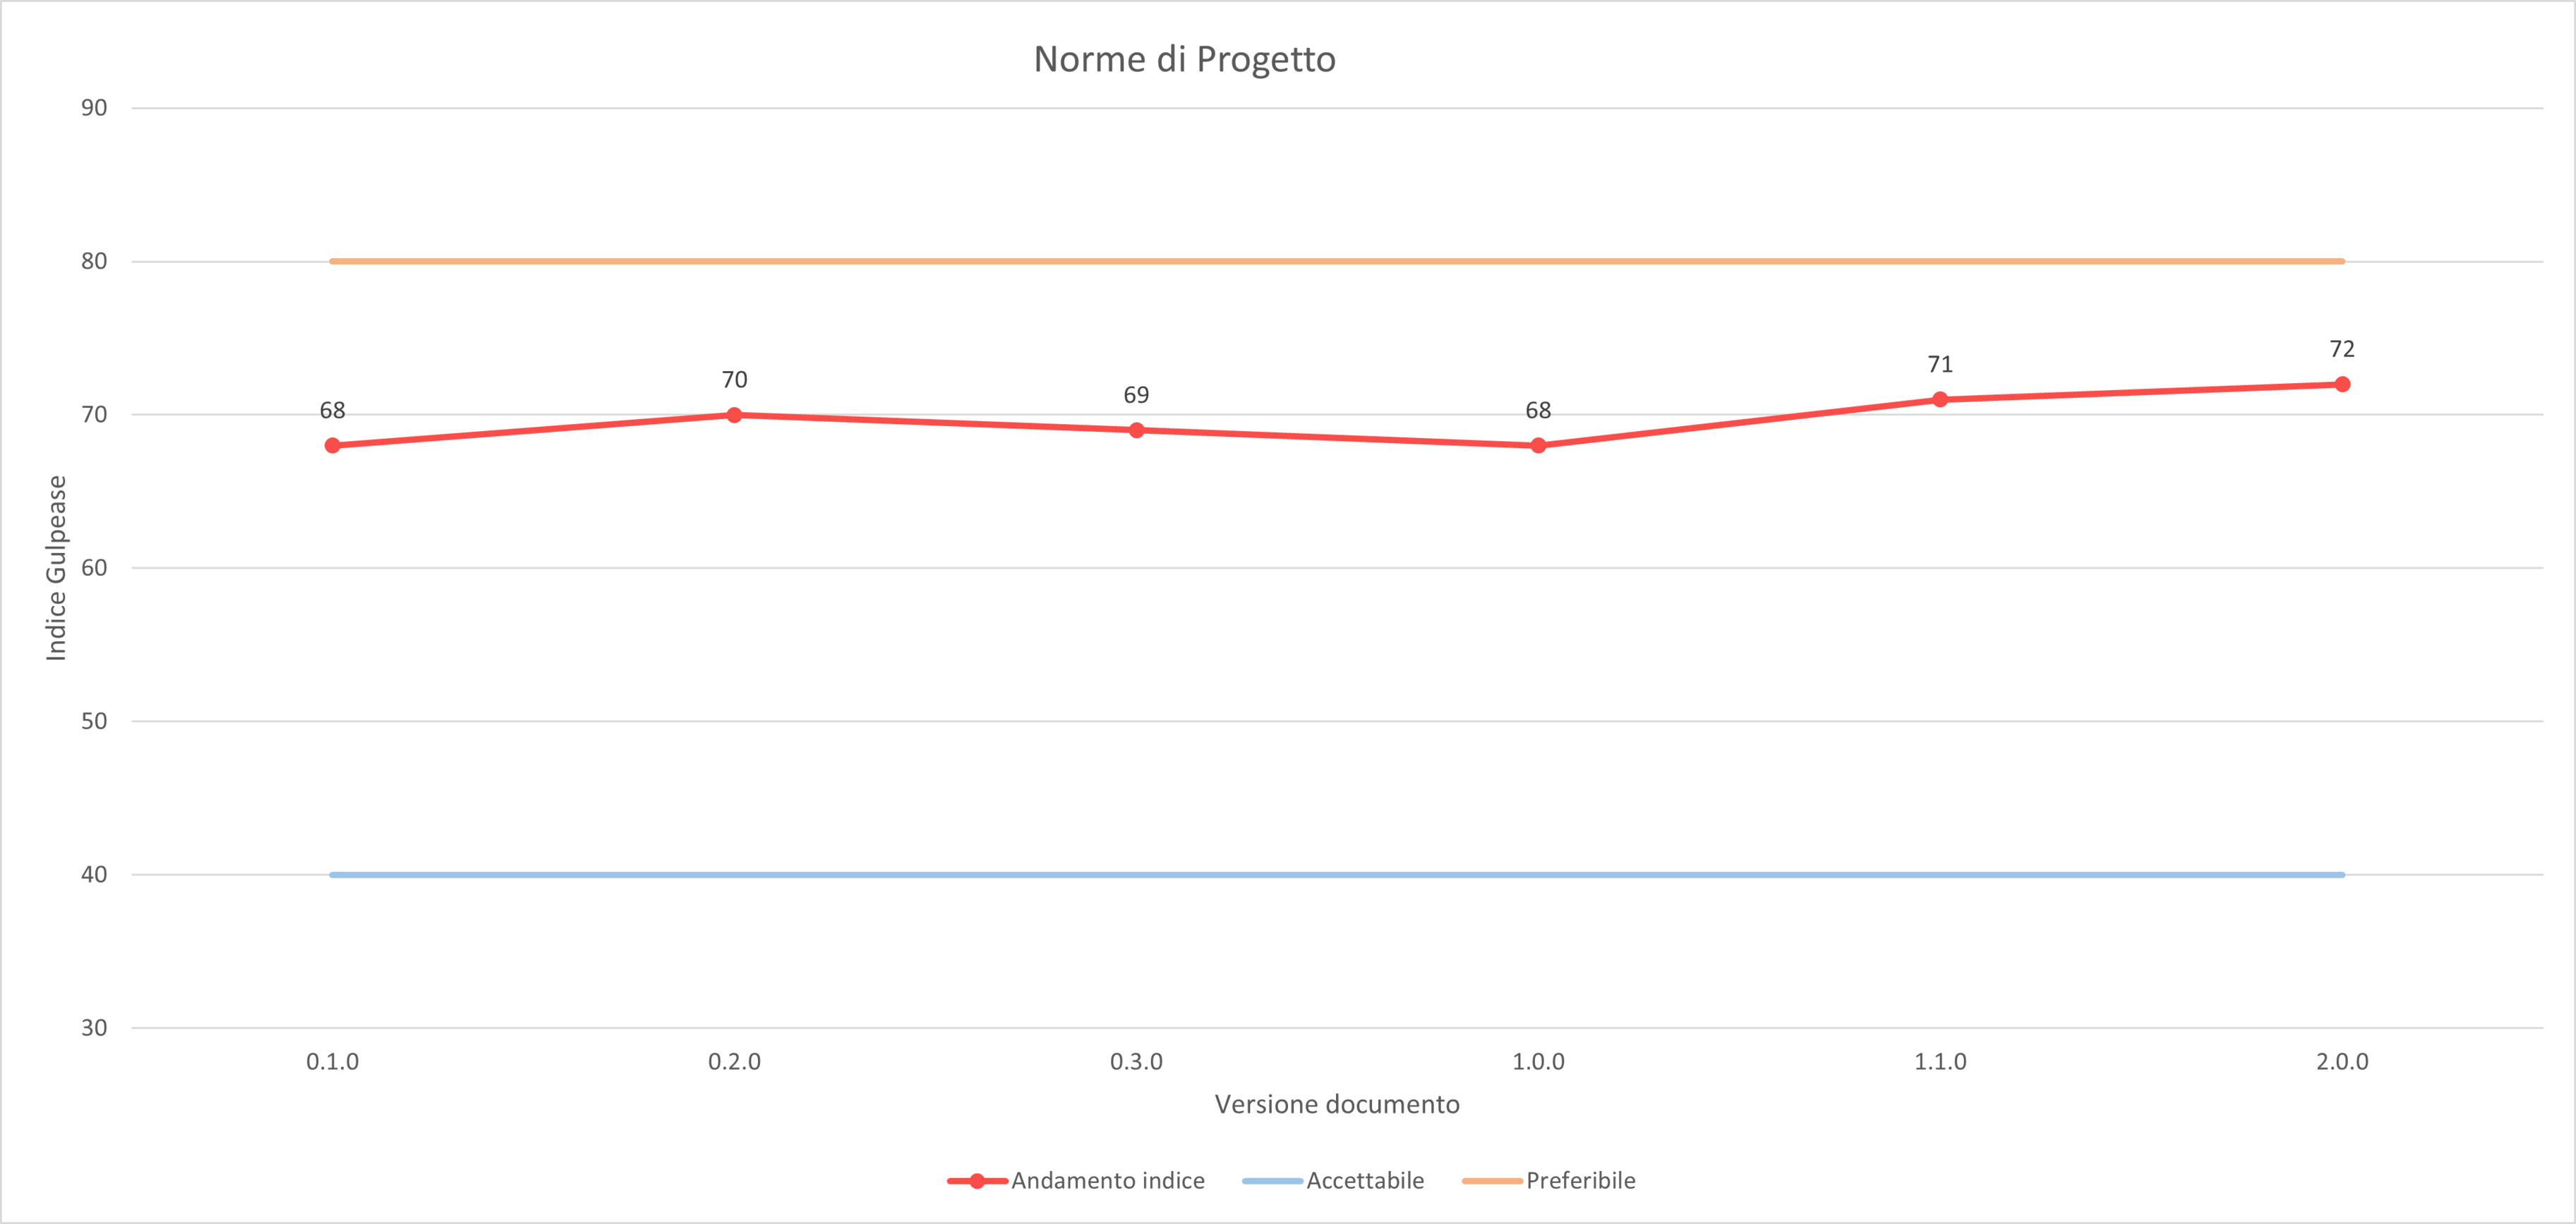
\includegraphics[scale=0.5]{sezioni/immagini/NormeGulpease.png}
    \centering
\end{figure}
\pagebreak
\begin{figure}[!ht]
    \caption{Indice di Gulpease: \textit{Piano di Progetto}}
    \vspace{10px}
    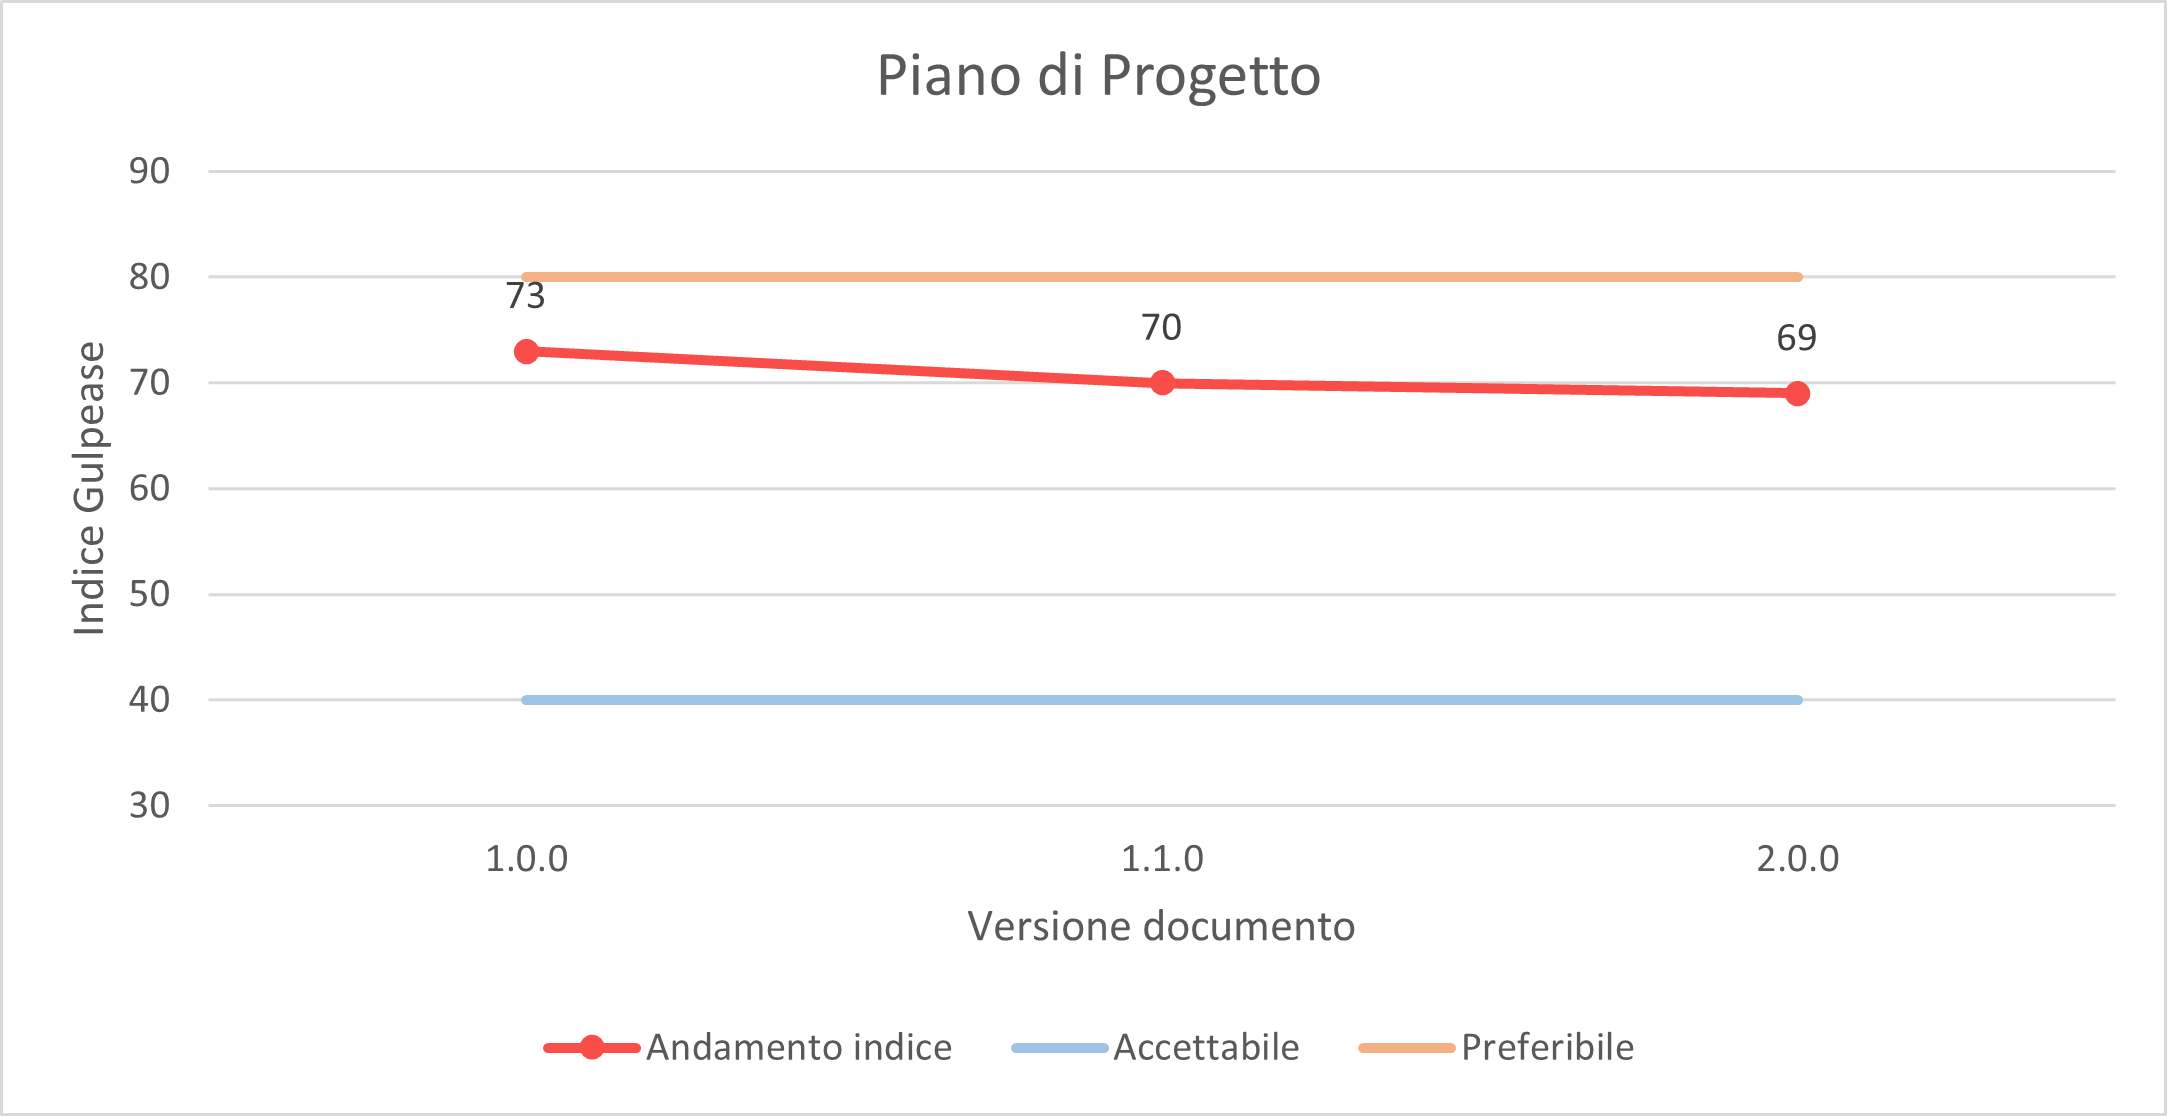
\includegraphics[scale=0.5]{sezioni/immagini/PianoProgettoGulpease.png}
    \centering
\end{figure}

\begin{figure}[!ht]
    \caption{Indice di Gulpease: \textit{Analisi dei Requisiti}}
    \vspace{10px}
    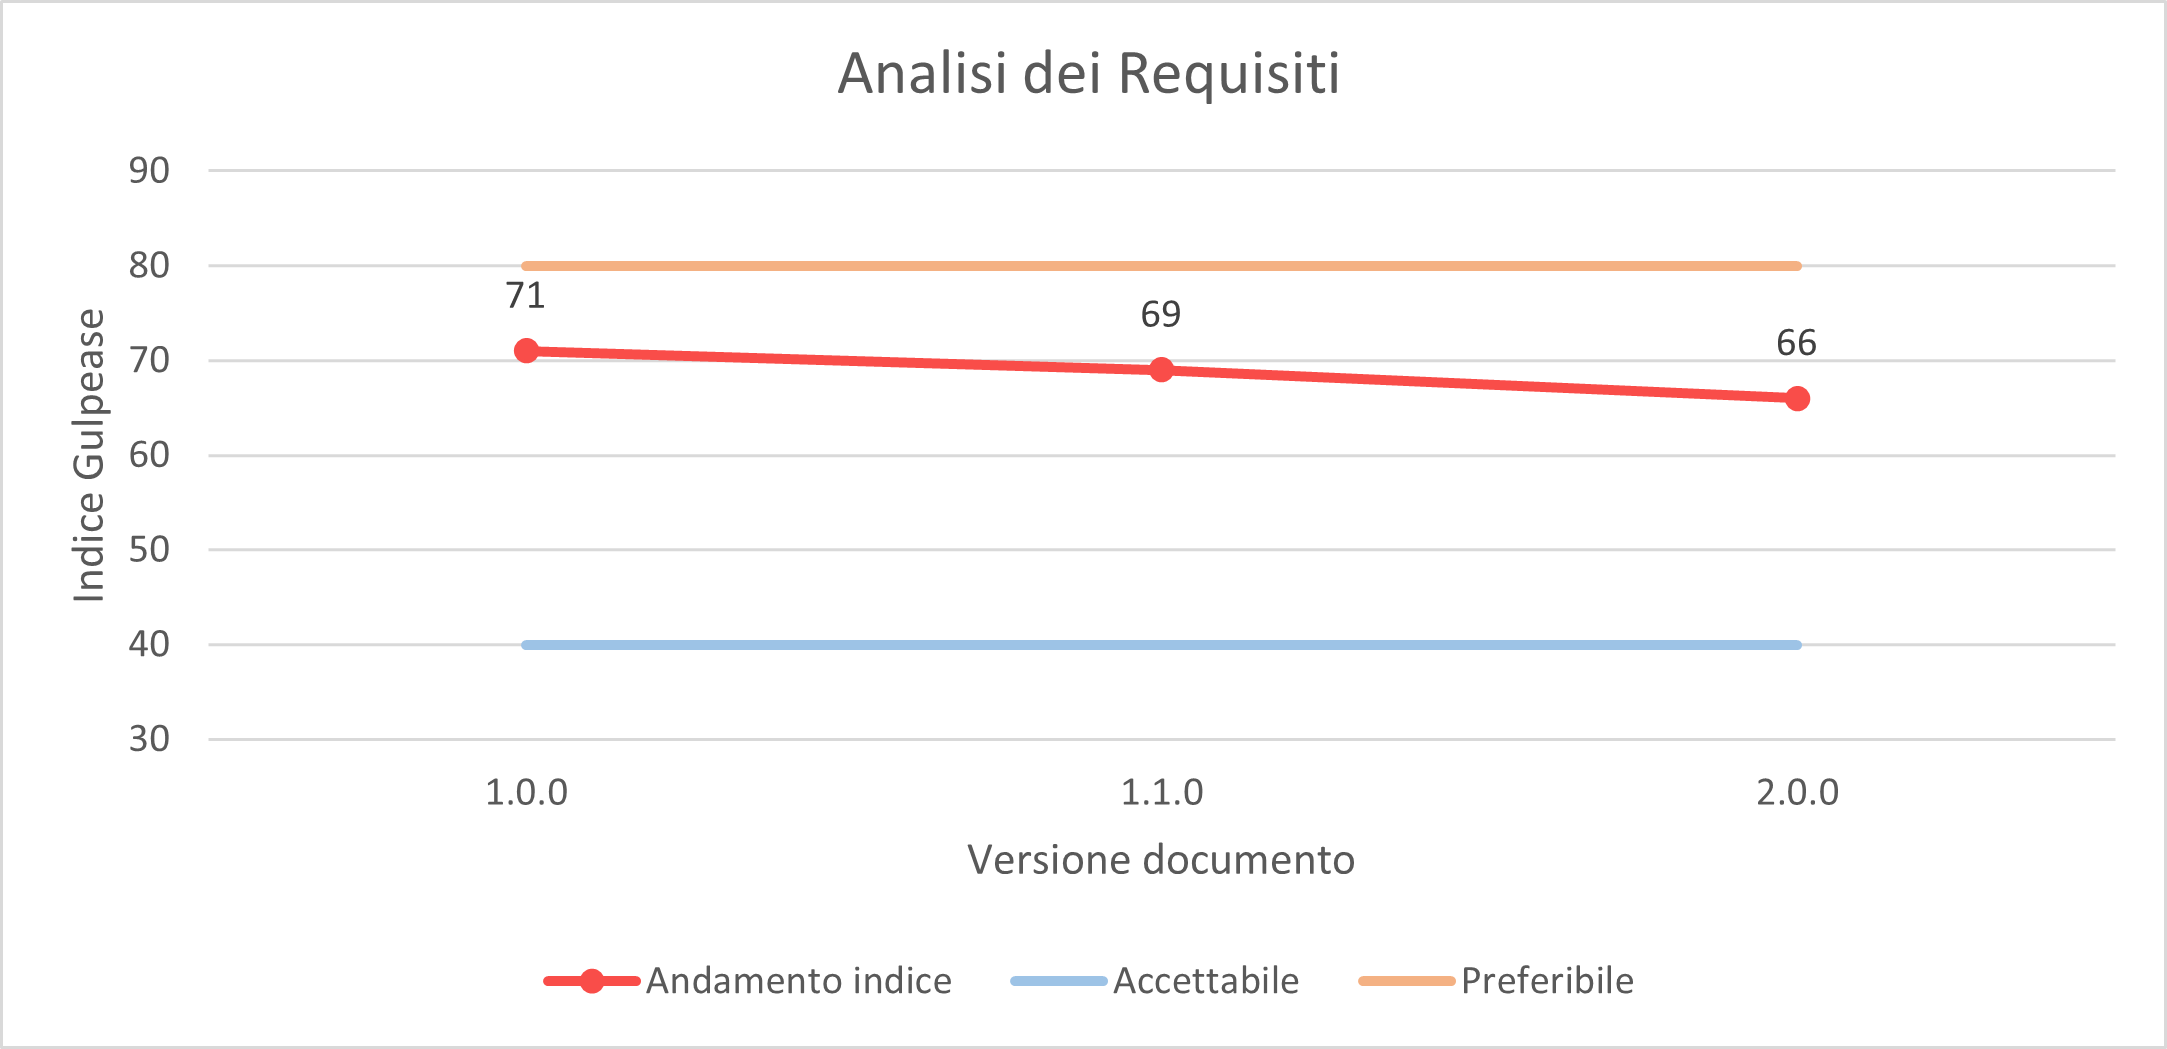
\includegraphics[scale=0.5]{sezioni/immagini/AnalisiGulpease.png}
    \centering
\end{figure}

\begin{figure}[!ht]
    \caption{Indice di Gulpease: \textit{Piano di Qualifica}}
    \vspace{10px}
    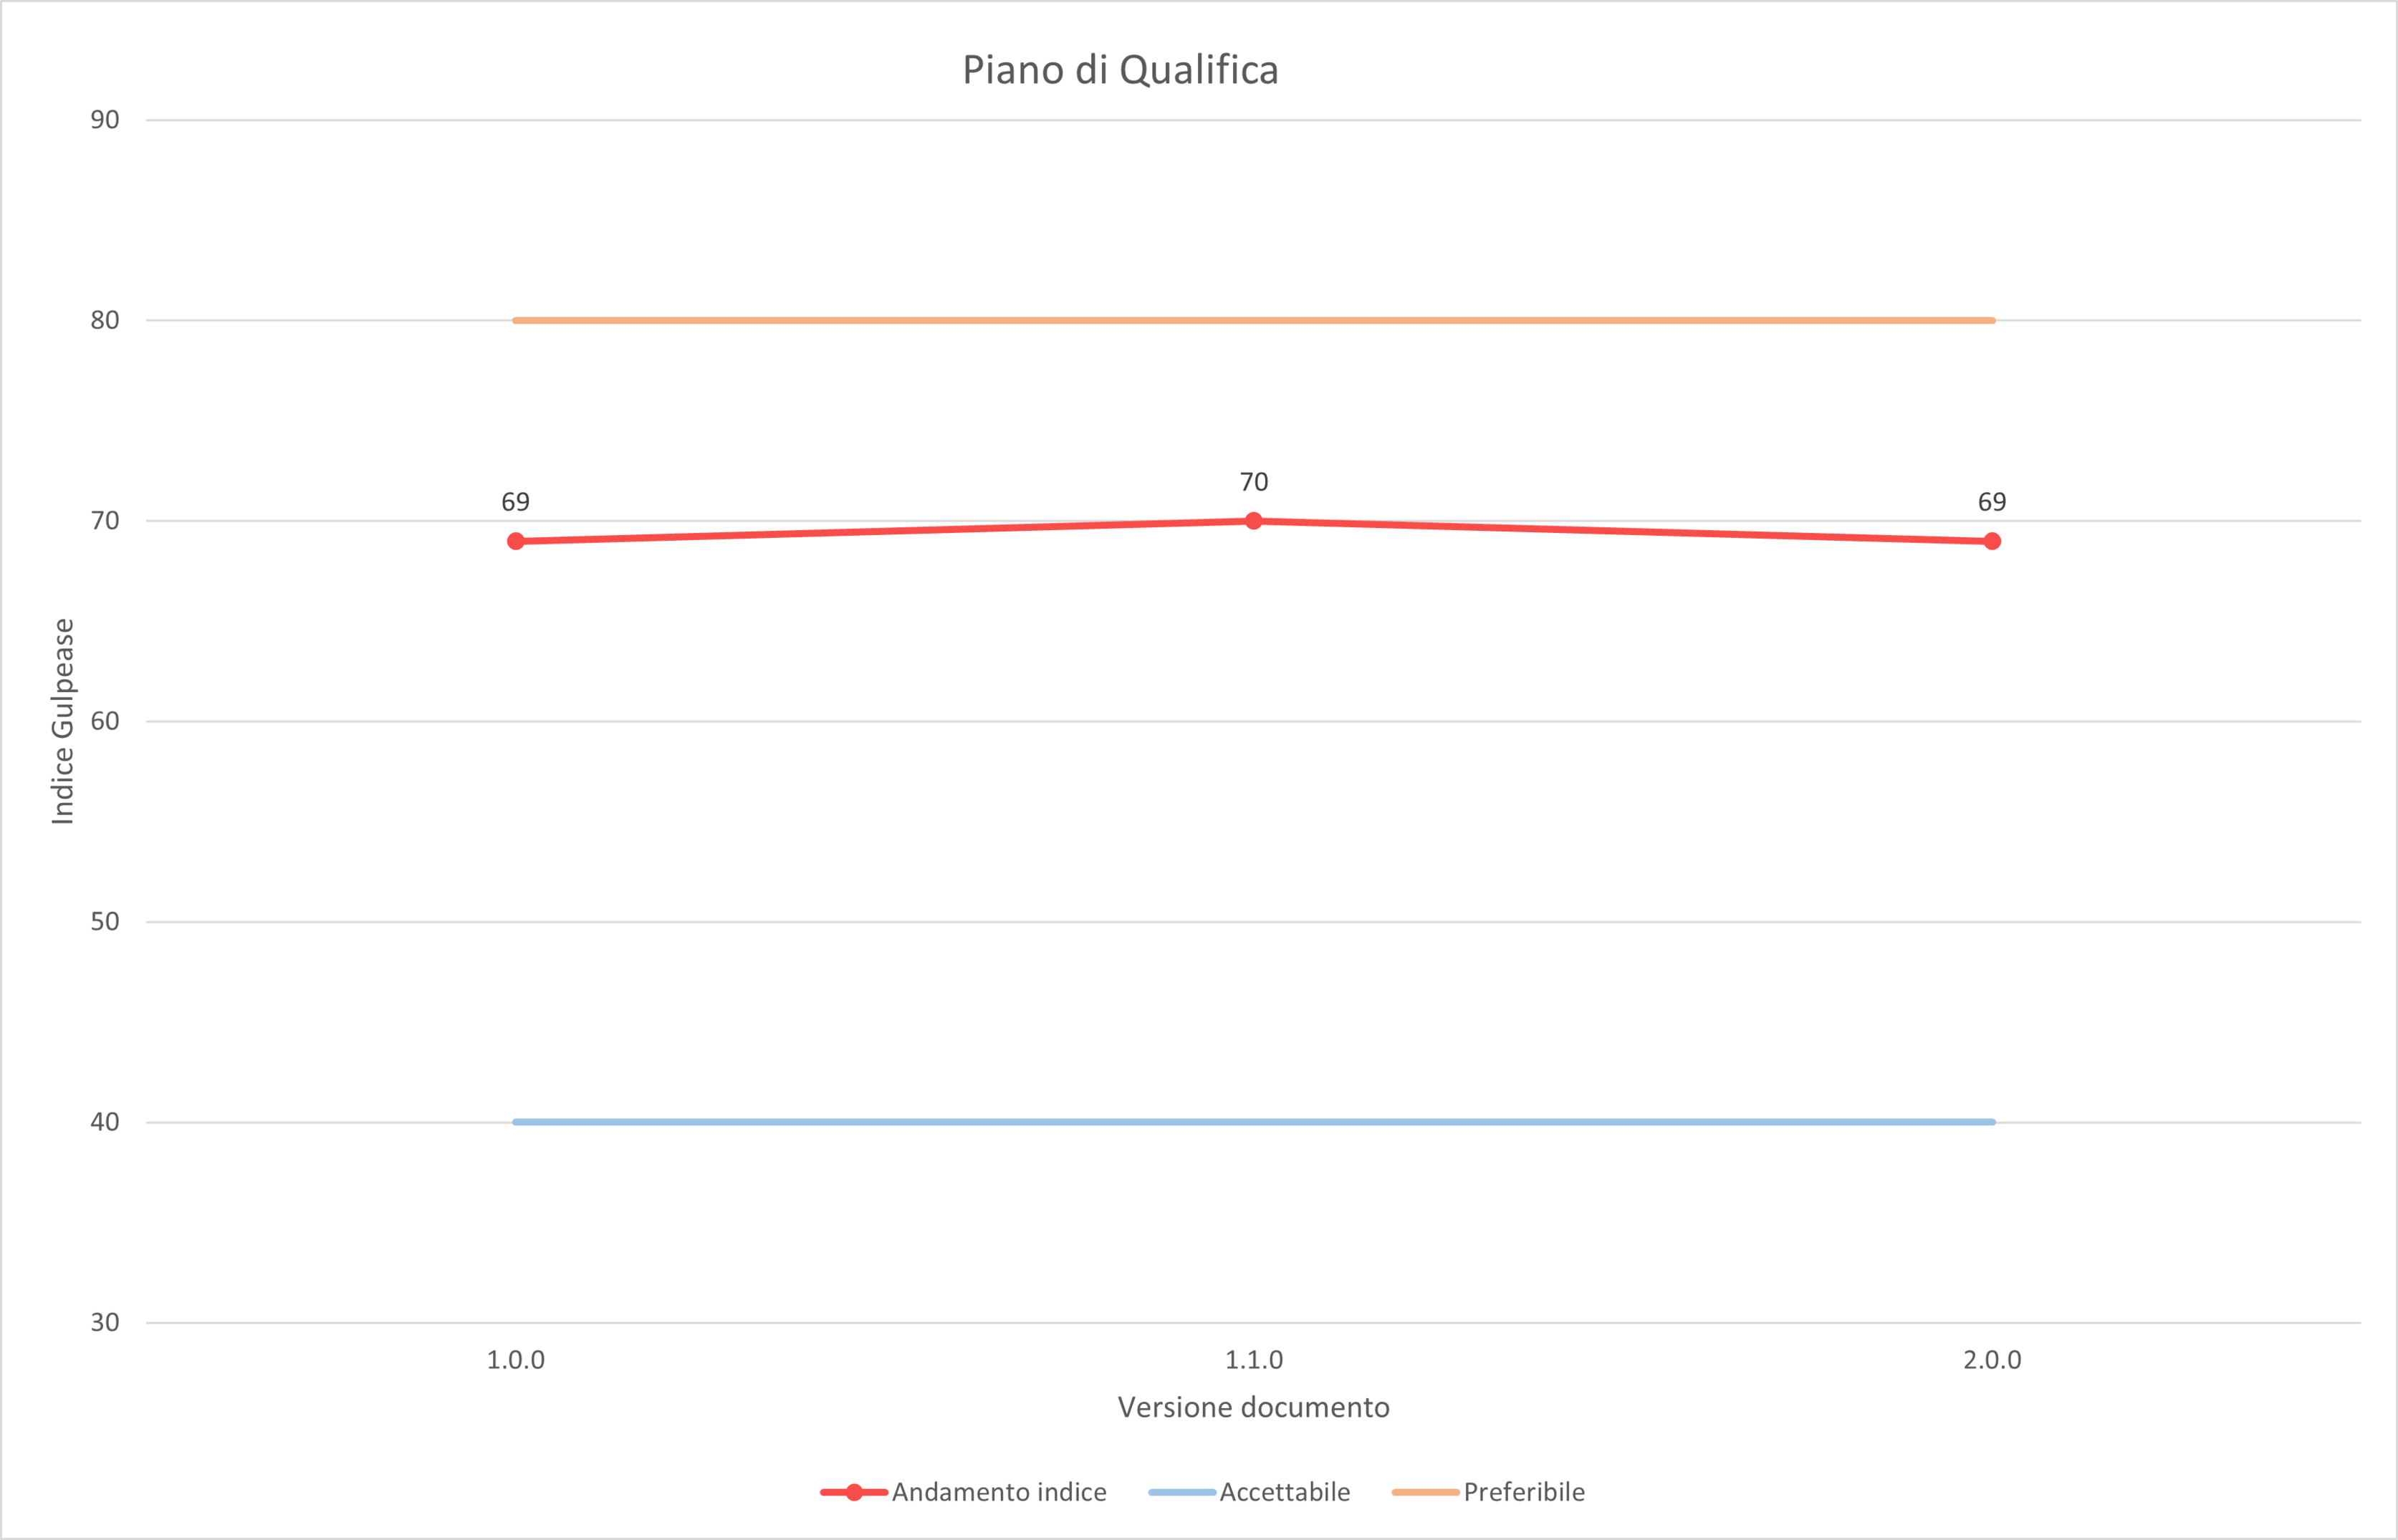
\includegraphics[scale=0.5]{sezioni/immagini/PianoQualificaGulpease.png}
    \centering
\end{figure}
\pagebreak
\begin{figure}[!ht]
    \caption{Indice di Gulpease: \textit{Studio di Fattibilità}}
    \vspace{10px}
    \includegraphics[scale=0.5]{sezioni/immagini/FattibilitàGulpease.png}
    \centering
\end{figure}

\begin{figure}[!ht]
    \caption{Indice di Gulpease: \textit{Glossario}}
    \vspace{10px}
    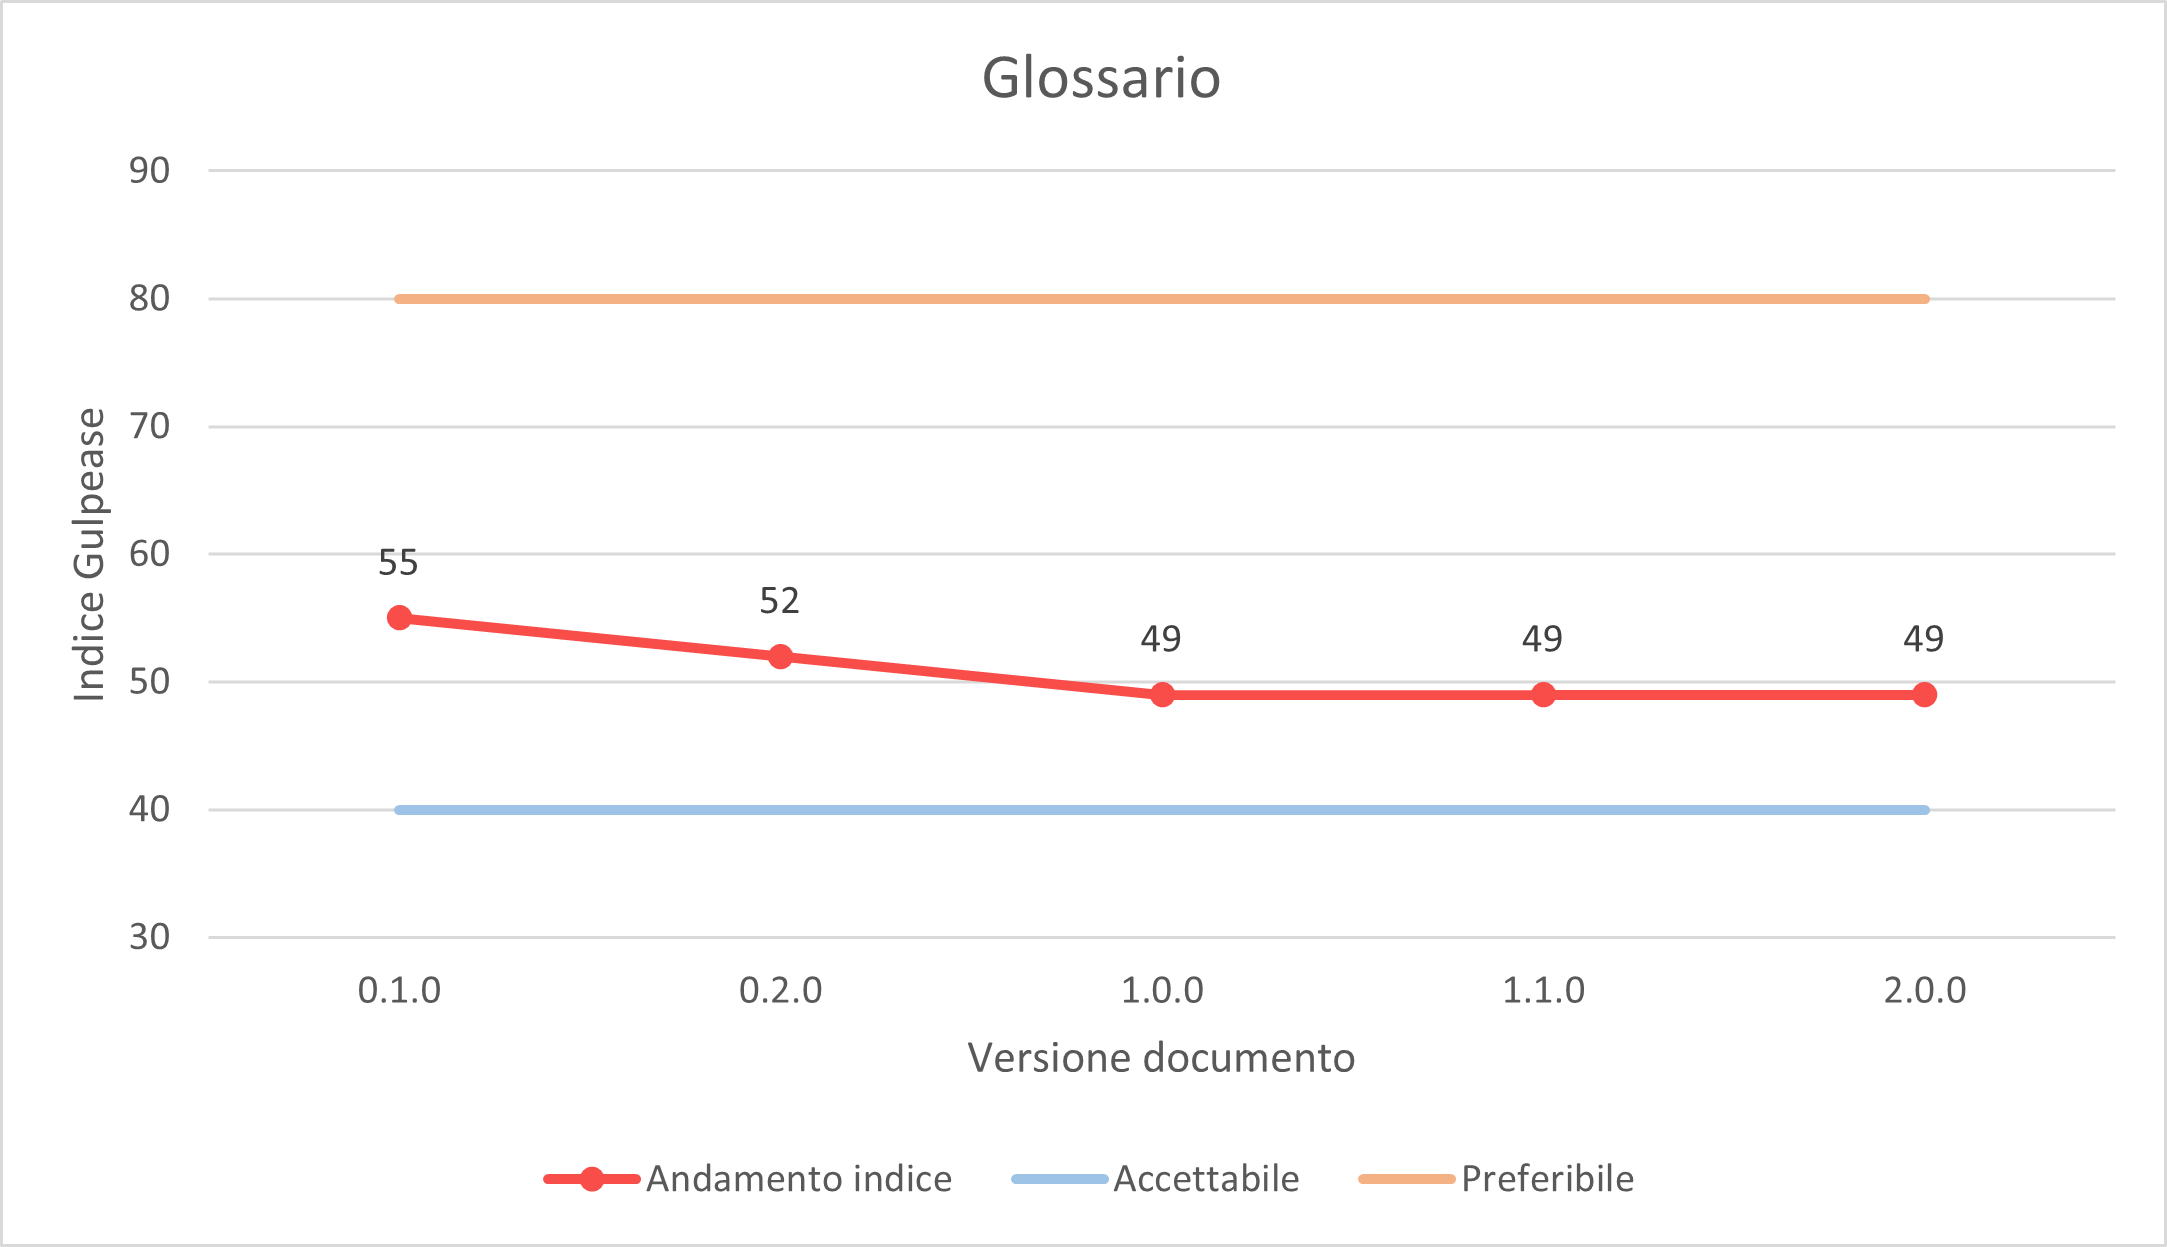
\includegraphics[scale=0.5]{sezioni/immagini/GlossarioGulpease.png}
    \centering
\end{figure}

\subsubsection{MPR11 - Correttezza ortografica}
\begin{figure}[!ht]
    \caption{Correttezza ortografica}
    \vspace{10px}
    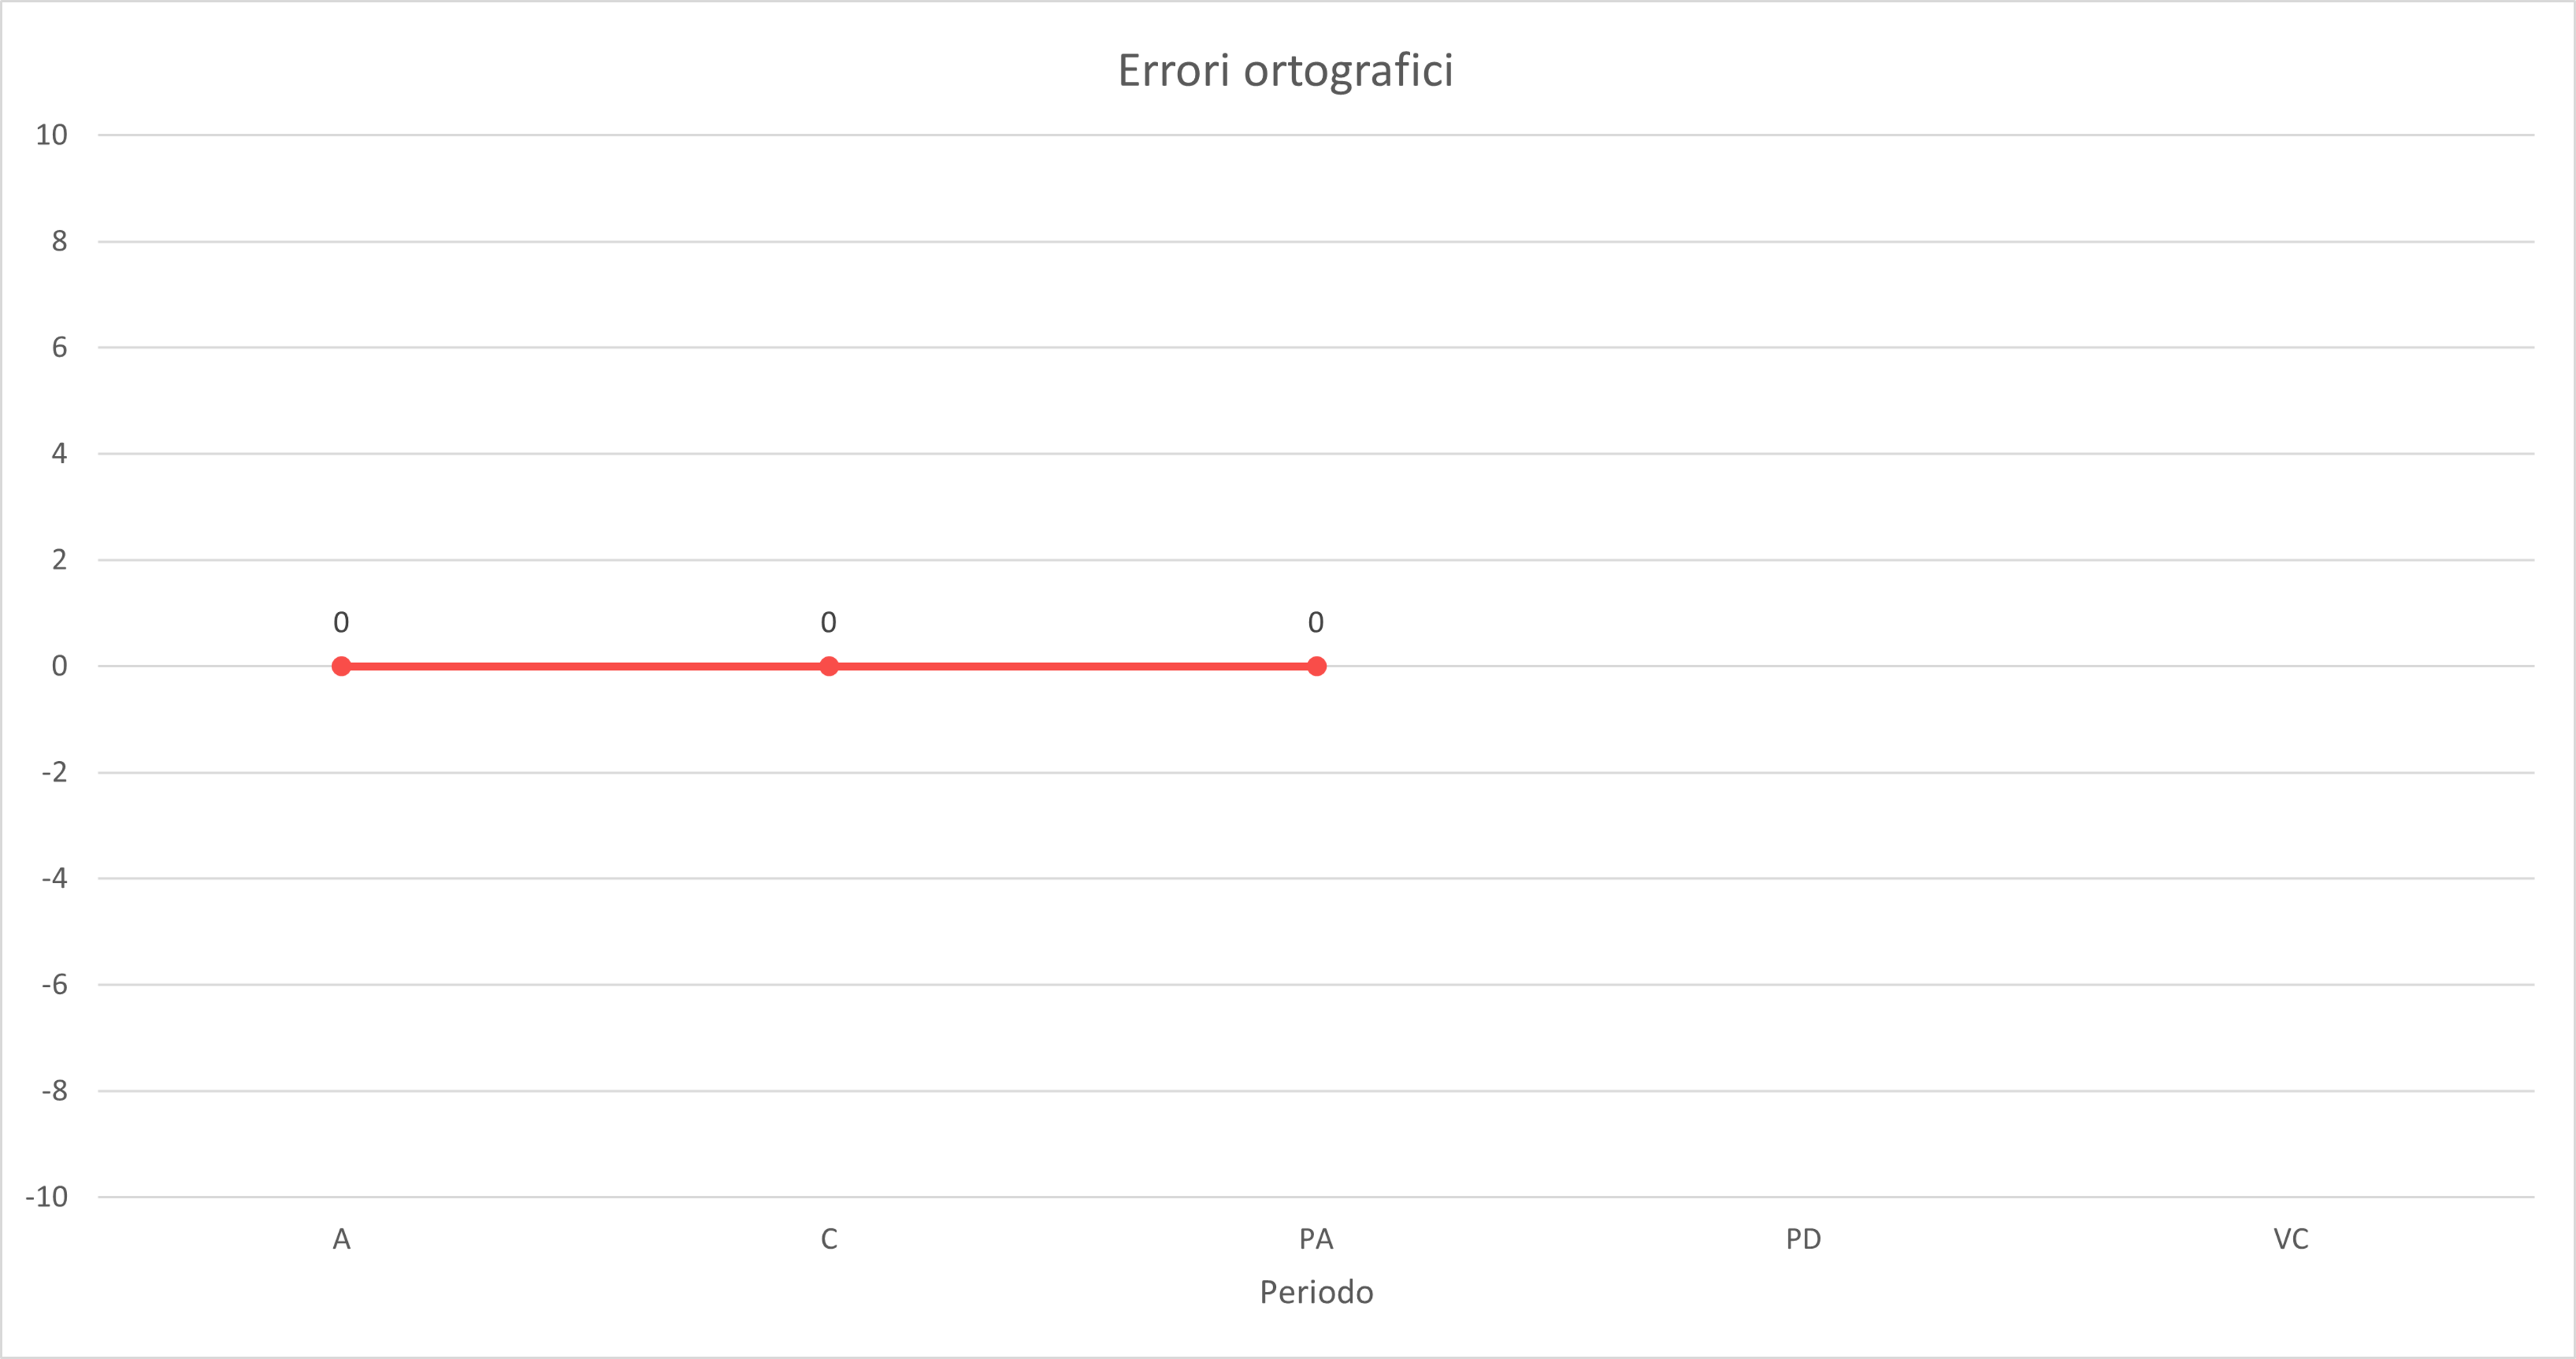
\includegraphics[scale=0.5]{sezioni/immagini/CorrettezzaOrtografica.png}
    \centering
\end{figure}
\pagebreak
\subsubsection{MPR12 - PMS (Percentuale di metriche soddisfatte)}
\begin{figure}[!ht]
    \caption{Percentuale di metriche soddisfatte}
    \vspace{10px}
    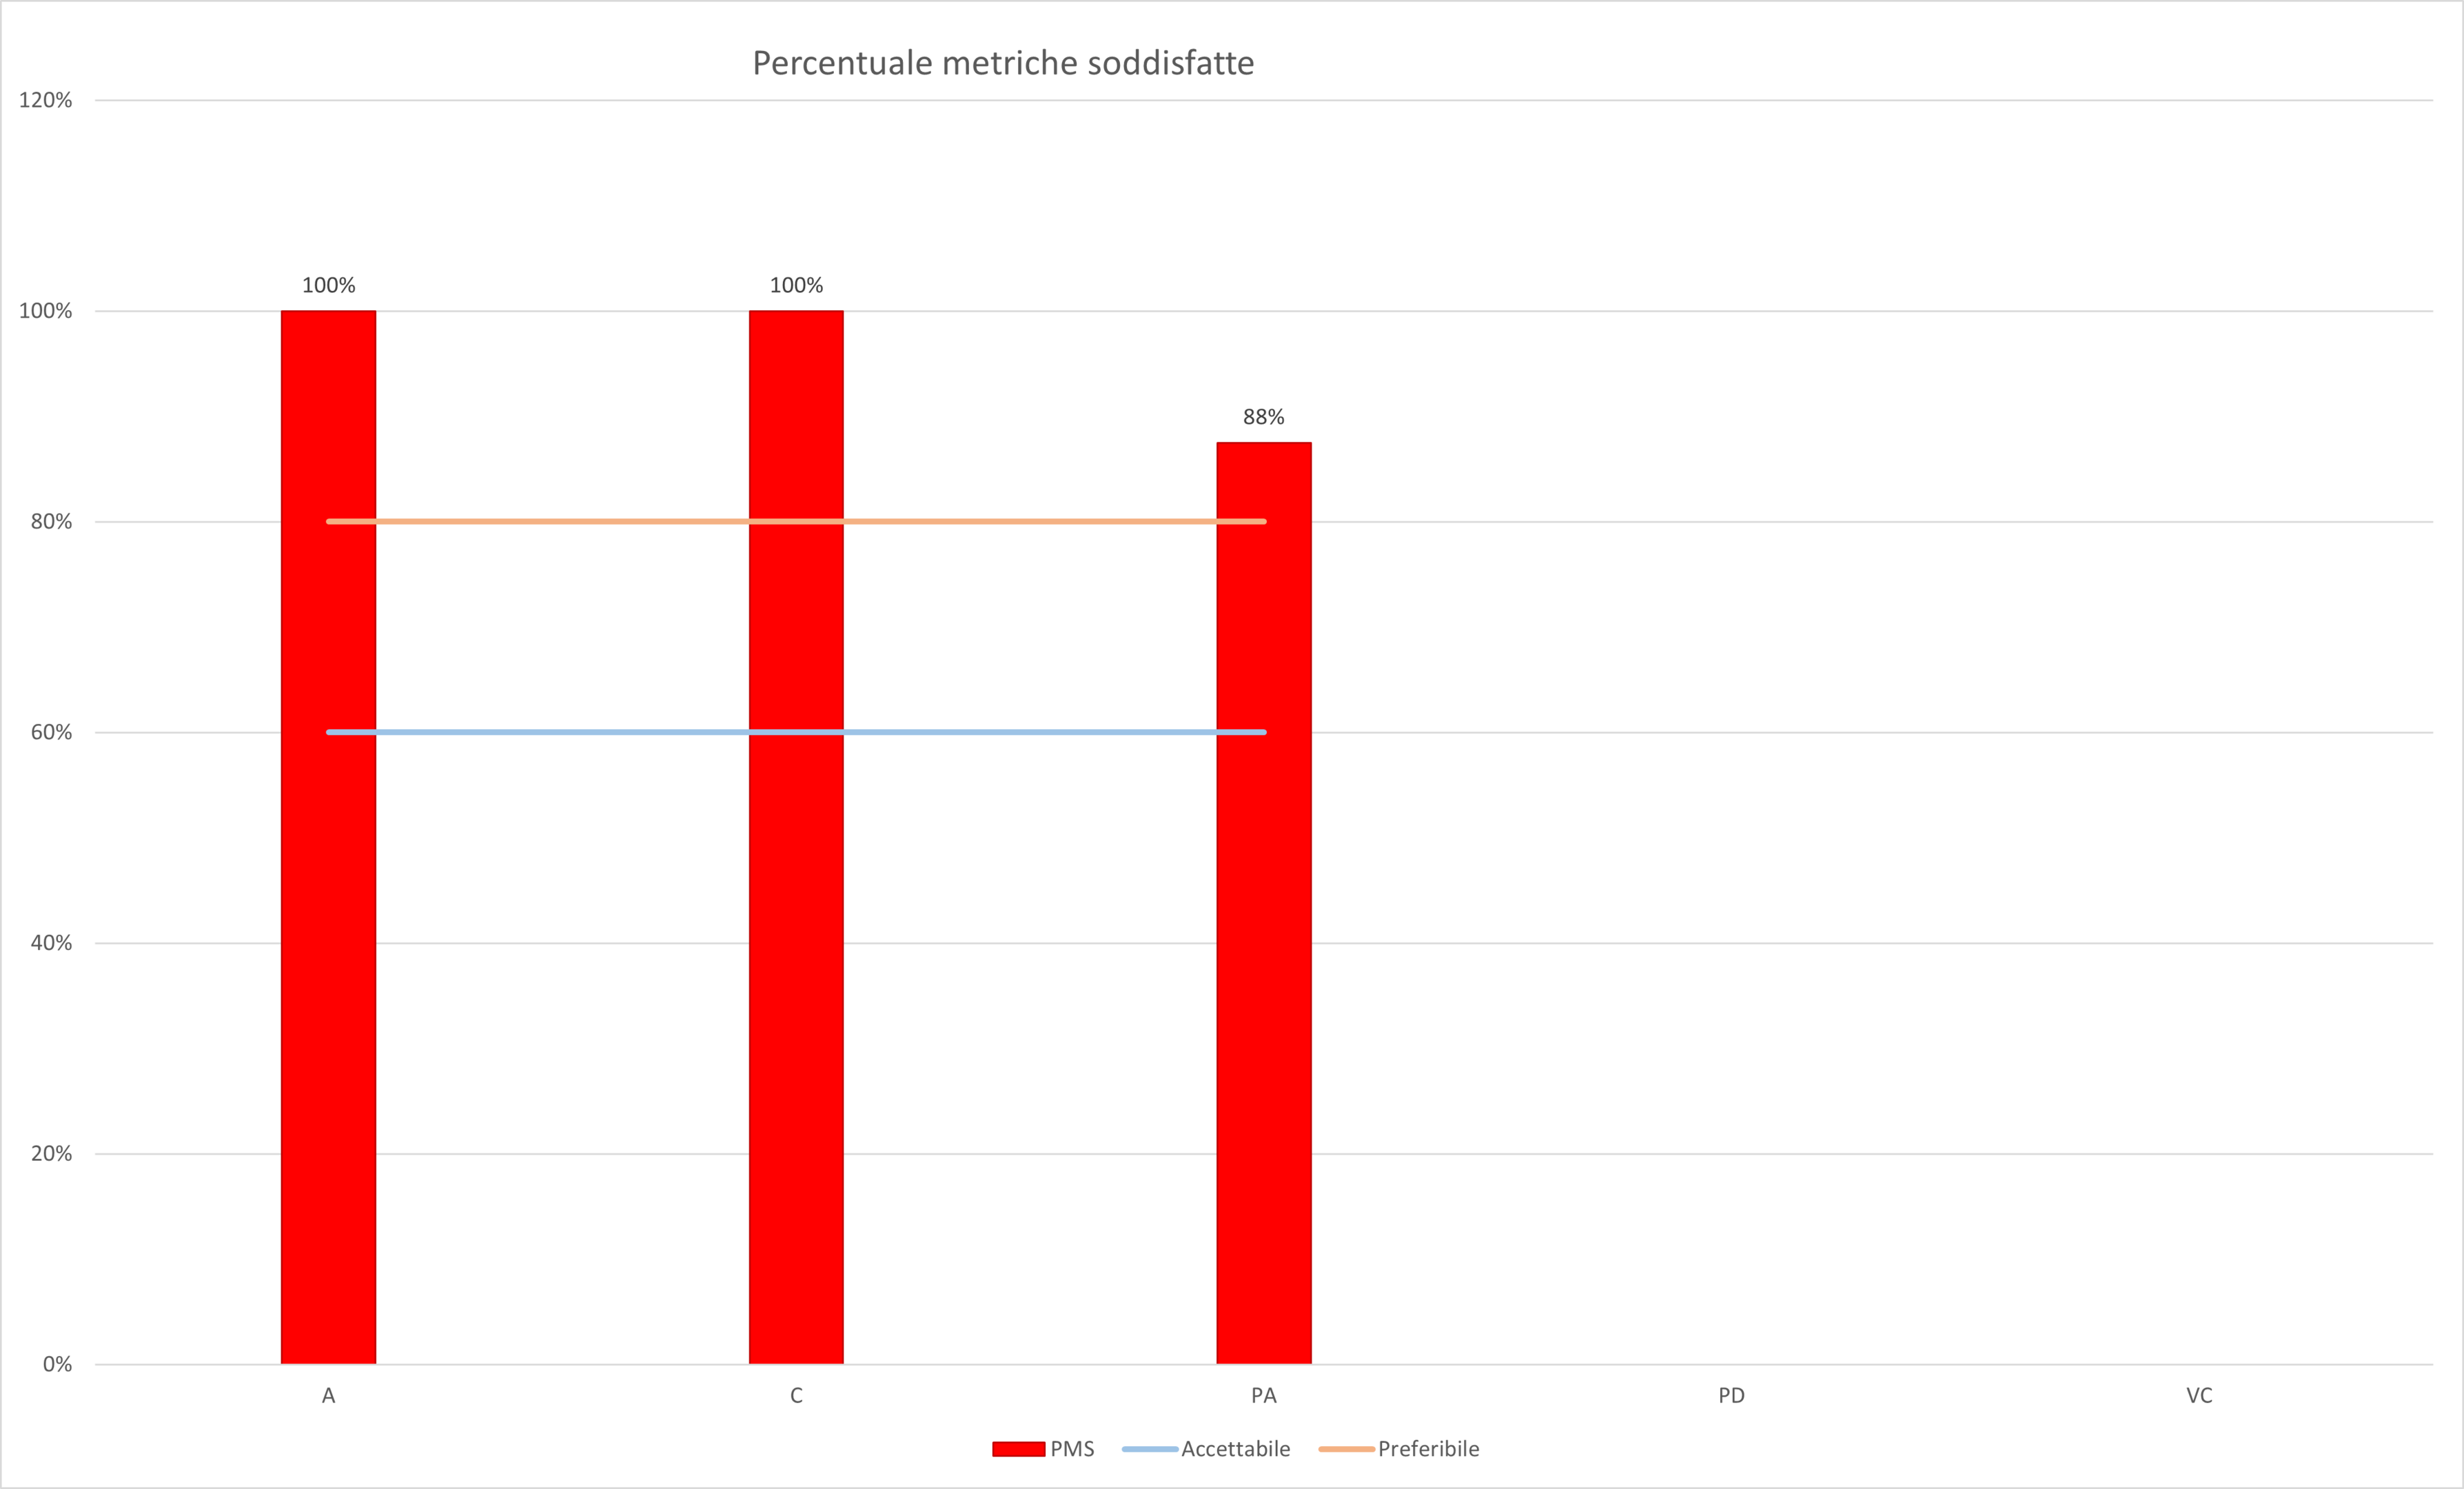
\includegraphics[scale=0.5]{sezioni/immagini/MetricheSoddisfatte.png}
    \centering
\end{figure}
\newpage